\documentclass{beamer}
%\usepackage[none]{hyphenat}
\usepackage{multicol}

% we can use a theme for our presentation
% \usetheme{Warsaw}
\usetheme[progressbar=frametitle]{metropolis}


\setbeamertemplate{frame numbering}[fraction]
\useoutertheme{metropolis}
\useinnertheme{metropolis}
\usefonttheme{metropolis}
\usecolortheme{spruce}
%\usecolortheme{crane}
\setbeamercolor{background canvas}{bg=white}

% we can also define our colour
% we can goto latexcolor.com to check many color values for latex
\definecolor{mygreen}{rgb}{.125,.5,.25}
\usecolortheme[named=mygreen]{structure}

% title, author institute, date: for the first title page
% this titlepage has to be created inside the document by using
% backlash titlepage
\title{Functions, Limits, Derivatives}
%\title[short title]{your title here}
%\subtitle{Subtitle Here}
\author{Kamaljeet Singh}
%\institute{institute name}
\institute{\large \textbf{Learning Outcomes}: \\[6pt] Identify properties of elementary functions (formed by composition of power, exponential, logarithmic, and trigonometric functions and their inverses).}
\date{}

\setbeamercovered{transparent=5}

\begin{document}
\metroset{block=fill}

% in beamer we create frames to hold all of our information
% a frame can contain a single or multiple slides that are part of our presentation
%\begin{frame}{title name of my slide}
\begin{frame}
% title page will show info taken from preamble: title, author, institute, date
\titlepage
\end{frame}

\begin{frame}[t]{Functions} \vspace{4pt}
\begin{block}{Definition of a Function}
\vspace{0.5em}
A \textbf{function} $f$ is a rule that assigns to each element $x$ in a set $D$ exactly one element, called $f(x)$, in a set $E$.
\vspace{0.5em}
\end{block}

\vspace{10pt}
Set $D$ is called the 
\only<1>{ \line(1,0){50} }
\only<2>{\textcolor{magenta}{domain}}
 \, of the function.\\[10pt]

Set $E$ is called the 
\only<1>{ \line(1,0){50} }
\only<2>{\textcolor{magenta}{range}}
\, of the function.

\end{frame}


\begin{frame}{Your Very First Flash Card} \vspace{10pt}
\begin{columns}[onlytextwidth]
\column{0.4\textwidth}
$\sqrt{x^2}=$\\[10pt]
\begin{enumerate}[(A)]
\item $x$
\item $-x$
\item $|x|$
\item undefined
\end{enumerate}
\column{0.6\textwidth}
\only<3>{
$\sqrt{x^2}=
\begin{cases}
-x, & x<0 \\
x, & x \geq 0
\end{cases}$\\[10pt]}
\only<2->{
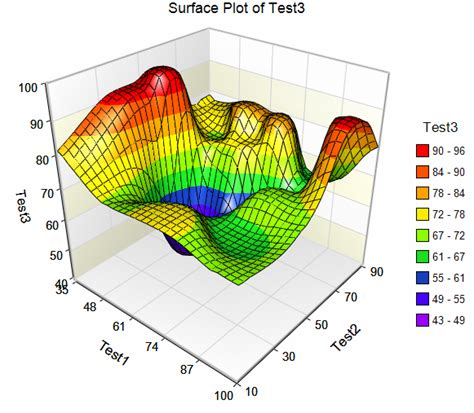
\includegraphics[scale=0.25]{plot1}
}
\end{columns}
\end{frame}

\begin{frame}[t]{Parent Functions} \vspace{4pt} 
You should be able to identify by name and sketch a graph of each of the following parent functions.
\begin{enumerate}
\begin{multicols}{3}
\item $y=x$
\item $y=|x|$
\item $y=x^2$
\item $y=x^3$
\item $y=x^b$
\onslide<2->{
\item $y=\sqrt{x}$
\item $y=\sqrt[3]{x}$
\item $y=\frac{1}{x}$
\item $y=2^x$
\item $y=e^x$
}
\onslide<3->{
\item $y=\ln x$
\item $y=\frac{1}{1+e^{-x}}$
\item $y=\sin x$
\item $y=\cos x$
\item $y=\tan x$ }
\end{multicols}
\end{enumerate}
\end{frame}

\begin{frame}[standout]
\flushleft
Homework: p.342 \#7-21
\end{frame}

\end{document}
